\documentclass[UTF8,a4paper,11pt]{ctexart}

\usepackage[margin=2.2cm]{geometry}
\usepackage{graphicx}
\usepackage{booktabs}
\usepackage{multirow}
\usepackage{array}
\usepackage{xcolor}
\usepackage{hyperref}
\usepackage{amsmath}
\usepackage{subcaption}
\usepackage{float}
\usepackage{enumitem}

\graphicspath{{assets/}}
\hypersetup{
    colorlinks=true,
    linkcolor=blue!55!black,
    urlcolor=blue!55!black,
    citecolor=blue!55!black
}

\title{基于 VGGT、Bundle Adjustment 与 3D Gaussian Splatting 的多视角三维重建}
\author{计算机视觉大作业初步报告}
\date{\today}

\begin{document}
\maketitle

\begin{abstract}
本项目面向无标定多视角图像的三维重建与实时渲染任务，搭建了从 VGGT 相机与点云估计、自实现 Bundle Adjustment（BA）优化，到 3D Gaussian Splatting（3DGS）训练和渲染评估的完整实验流水线。当前已经在 \texttt{scene}、\texttt{1-human}、\texttt{2-human} 三组数据上完成 VGGT、BA 与官方 3DGS 实验。实验表明，自实现 BA 可显著降低多视角重投影误差；在 \texttt{scene} 场景上，BA 后官方 3DGS 的 PSNR 从 20.73 dB 提升至 22.47 dB，SSIM 从 0.754 提升至 0.820，LPIPS 从 0.247 降至 0.197。针对 human 场景，进一步采用更高密度 VGGSfM tracks、mask 白底合成和固定 8 视角测试集后，\texttt{1-human} 达到 26.44 dB / 0.959 SSIM / 0.031 LPIPS，\texttt{2-human} 达到 28.62 dB / 0.968 SSIM / 0.024 LPIPS。自实现 3DGS 当前效果较差，仅作为失败分析展示；最终效果展示以官方 3DGS 结果为主。
\end{abstract}

\section{问题定义与系统流程}

本大作业要求在没有给定相机标定的情况下，仅使用场景多视角图像完成三维重建与实时交互渲染。整体任务可分为三个核心问题：

\begin{enumerate}[leftmargin=2em]
    \item 从多视角图像估计每张图像的相机内参、外参和初始三维点云。
    \item 在初始几何结果上进行 BA，联合优化相机外参与三维点位置，提升多视角几何一致性。
    \item 以优化后的相机和点云作为 3DGS 初始化，训练可实时渲染的新视角表示，并用图像指标和可视化结果评估质量。
\end{enumerate}

项目的实际流水线如下：

\[
\texttt{images}
\rightarrow \texttt{VGGT export}
\rightarrow \texttt{Reconstruction.npz}
\rightarrow \texttt{custom BA}
\rightarrow \texttt{Reconstruction.npz}
\rightarrow \texttt{official/custom 3DGS}
\rightarrow \texttt{rendering + metrics}.
\]

各阶段统一使用 \texttt{src/data/reconstruction.py} 中的 \texttt{Reconstruction} 数据结构传递信息，包含图像名、图像尺寸、相机内参、OpenCV camera-from-world 外参、稀疏三维点、颜色、置信度，以及 BA 所需的观测图。这样可以避免各阶段使用临时格式造成坐标系和索引不一致。

\begin{figure}[H]
    \centering
    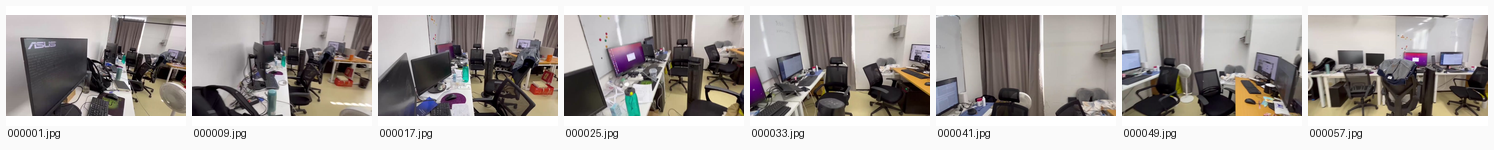
\includegraphics[width=0.95\linewidth]{scene_input_montage.png}
    \caption{\texttt{scene} 场景输入多视角图像示例。}
    \label{fig:scene-input}
\end{figure}

\begin{figure}[H]
    \centering
    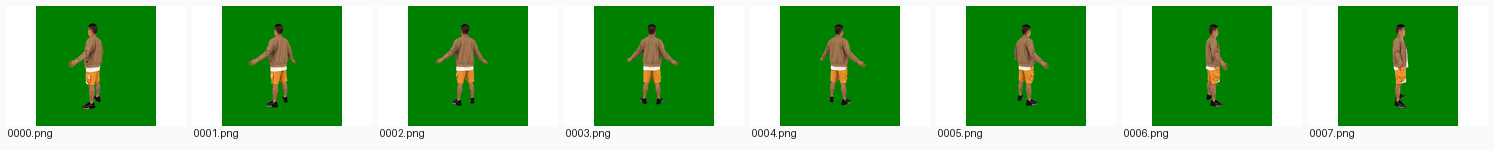
\includegraphics[width=0.95\linewidth]{1-human_input_montage.png}
    \caption{\texttt{1-human} 场景输入图像示例。该数据包含纯绿色背景，前景人体占画面比例较小，对 3DGS 训练和图像指标解释都有明显影响。}
    \label{fig:human-input}
\end{figure}

\section{VGGT 初始重建结果}

VGGT 阶段负责从未标定图像中预测相机参数、稠密点图和跨视角 tracks。导出脚本进一步筛选可见性、置信度和重投影误差，形成稀疏观测图。为了在没有真值相机和真值点云时评估 VGGT 的几何质量，本报告使用自监督多视角重投影一致性指标：

\[
e_{ij} = \left\| \pi(K_i, R_i, t_i, X_j) - x_{ij} \right\|_2,
\]

其中 \(X_j\) 是三维点，\(x_{ij}\) 是该点在第 \(i\) 张图像中的 track 观测，\(\pi\) 是针孔投影函数。统计所有有效观测的 RMSE、median、P90 等数值，可以反映当前相机和点云对 VGGT track 的解释能力。

\begin{table}[H]
\centering
\caption{VGGT raw 重建统计与自监督重投影误差。}
\label{tab:vggt}
\begin{tabular}{lrrrrrr}
\toprule
场景 & 图像数 & 点数 & 观测数 & RMSE(px) & Median(px) & P90(px) \\
\midrule
\texttt{scene} & 64 & 9,760 & 116,725 & 3.82 & 2.80 & 6.42 \\
\texttt{1-human} & 16 & 7,667 & 57,446 & 3.58 & 2.49 & 6.16 \\
\texttt{2-human} & 16 & 7,421 & 59,191 & 3.25 & 2.16 & 5.61 \\
\bottomrule
\end{tabular}
\end{table}

从表 \ref{tab:vggt} 可以看到，三个场景的初始几何均达到可继续 BA 的程度，但 human 场景的图像数量少、前景区域小，并且纯绿色背景占据大部分像素。该数据特性会导致两个问题：第一，背景区域容易主导 3DGS 的图像损失和 SSIM；第二，前景人体几何点较稀疏，局部漂浮点会显著影响渲染观感。

\begin{figure}[H]
    \centering
    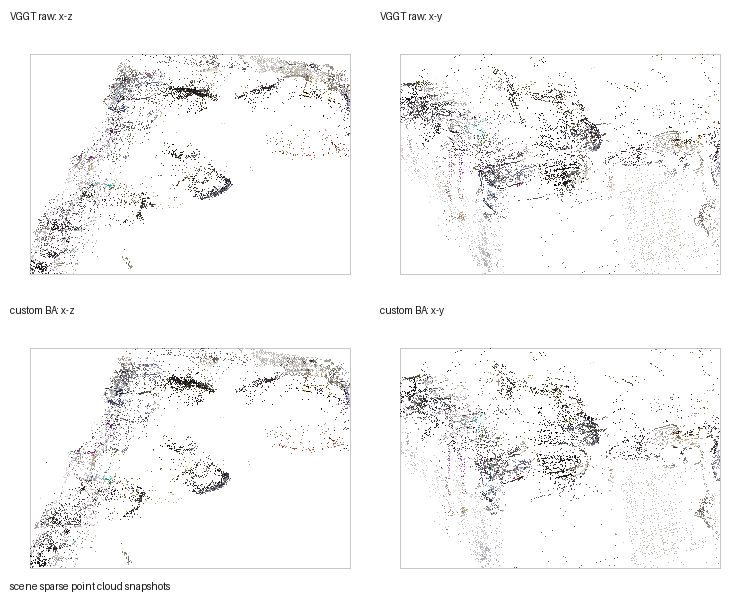
\includegraphics[width=0.72\linewidth]{scene_pointcloud_raw_ba.png}
    \caption{\texttt{scene} 稀疏点云 raw/BA 快照。点云快照主要用于检查几何尺度、离群点和结构分布。}
    \label{fig:scene-pcd}
\end{figure}

\section{Bundle Adjustment 优化结果}

自实现 BA 在 VGGT 初始结果上联合优化相机外参和三维点位置，内参在当前实验中固定。优化目标为鲁棒化重投影误差：

\[
\min_{\{R_i,t_i,X_j\}}
\sum_{(i,j)\in \mathcal{O}}
\rho \left(
\left\| \pi(K_i, R_i, t_i, X_j) - x_{ij} \right\|_2^2
\right),
\]

其中 \(\rho\) 为 Huber robust loss。当前实现采用两轮优化：第一轮用全部观测优化，随后根据重投影误差剔除离群观测；第二轮在清理后的观测图上继续优化。该流程既减少 VGGT tracks 中的错配影响，也保持了和下游 3DGS 兼容的相机/点云格式。

\begin{table}[H]
\centering
\caption{自实现 BA 前后重投影误差对比。}
\label{tab:ba}
\begin{tabular}{lrrrrrr}
\toprule
\multirow{2}{*}{场景} & \multicolumn{3}{c}{VGGT raw} & \multicolumn{3}{c}{Custom BA} \\
\cmidrule(lr){2-4}\cmidrule(lr){5-7}
 & RMSE & Median & P90 & RMSE & Median & P90 \\
\midrule
\texttt{scene} & 3.82 & 2.80 & 6.42 & 1.58 & 0.79 & 2.79 \\
\texttt{1-human} & 3.58 & 2.49 & 6.16 & 1.45 & 0.89 & 2.36 \\
\texttt{2-human} & 3.25 & 2.16 & 5.61 & 1.67 & 1.07 & 2.79 \\
\bottomrule
\end{tabular}
\end{table}

\begin{figure}[H]
    \centering
    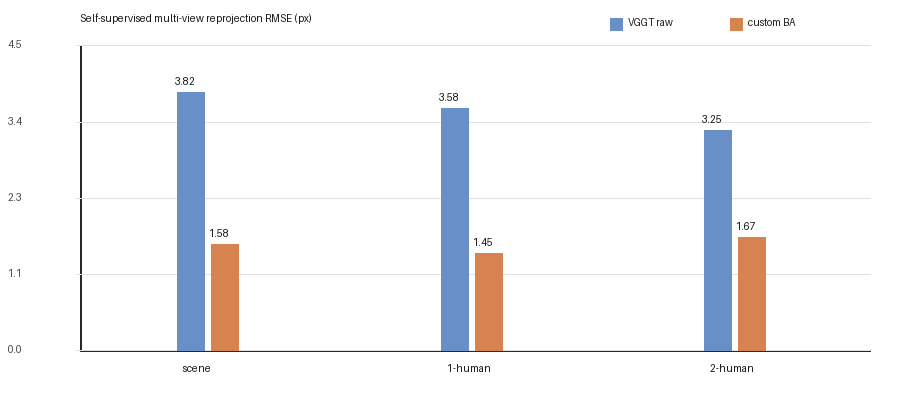
\includegraphics[width=0.78\linewidth]{ba_reprojection_rmse.png}
    \caption{VGGT raw 与 custom BA 的多视角重投影 RMSE 对比。}
    \label{fig:ba-rmse}
\end{figure}

\begin{table}[H]
\centering
\caption{BA 运行统计。}
\label{tab:ba-runtime}
\begin{tabular}{lrrrrr}
\toprule
场景 & BA时间(s) & 剔除观测 & 优化后点数 & 平均旋转变化(deg) & 收敛标记 \\
\midrule
\texttt{scene} & 122.10 & 4,280 & 9,679 & 0.301 & true \\
\texttt{1-human} & 93.06 & 650 & 8,202 & 0.117 & false \\
\texttt{2-human} & 61.87 & 1,594 & 7,252 & 0.052 & false \\
\bottomrule
\end{tabular}
\end{table}

BA 的主要结论是明确的：三个场景的重投影 RMSE 均显著下降，\texttt{scene} 从 3.82 px 降至 1.58 px；初始 human 实验中 \texttt{1-human} 从 3.58 px 降至 1.45 px，\texttt{2-human} 从 3.25 px 降至 1.67 px。进一步针对 human 场景重跑了高密度 VGGSfM tracks（\texttt{max\_query\_pts=1024}, \texttt{query\_frame\_num=16}）和 BA，结果见表 \ref{tab:human-hq-ba}。高密度设置显著增加了 tracks 和观测数量，并使 \texttt{2-human} 的 BA 后 RMSE 降至 1.36 px。

\begin{table}[H]
\centering
\caption{Human 场景高密度 tracks + BA 结果。}
\label{tab:human-hq-ba}
\begin{tabular}{lrrrrrr}
\toprule
场景 & 点数 & 观测数 & RMSE前 & RMSE后 & P90后 & BA时间(s) \\
\midrule
\texttt{1-human} & 18,183 & 138,917 & 3.39 & 1.53 & 2.52 & 195.6 \\
\texttt{2-human} & 17,678 & 143,966 & 3.07 & 1.36 & 2.21 & 153.0 \\
\bottomrule
\end{tabular}
\end{table}

\section{3D Gaussian Splatting 渲染结果}

本项目实现了一个自定义 3DGS 训练器，并额外接入官方 3DGS 仓库作为主要渲染基线。当前自实现 3DGS 在 \texttt{scene} 上可以训练并导出 checkpoint，但渲染结果明显模糊和扭曲，PSNR/SSIM 也显著低于官方实现。因此后续报告中将自实现 3DGS 作为工程探索和失败分析，最终效果展示主要使用官方 3DGS。

\begin{table}[H]
\centering
\caption{\texttt{scene} 场景 3DGS 定量结果。测试集为 8 个 hold-out 视角，训练迭代数为 10,000。}
\label{tab:gs-scene}
\begin{tabular}{lrrrr}
\toprule
方法 & Test视角数 & PSNR$\uparrow$ & SSIM$\uparrow$ & LPIPS$\downarrow$ \\
\midrule
VGGT raw + official 3DGS & 8 & 20.73 & 0.754 & 0.247 \\
Custom BA + official 3DGS & 8 & \textbf{22.47} & \textbf{0.820} & \textbf{0.197} \\
VGGT raw + random init official 3DGS & 8 & 20.32 & 0.742 & 0.264 \\
Custom BA + random init official 3DGS & 8 & 21.98 & 0.806 & 0.215 \\
Custom BA + self 3DGS & 8 & 16.40 & 0.570 & -- \\
\bottomrule
\end{tabular}
\end{table}

\begin{figure}[H]
    \centering
    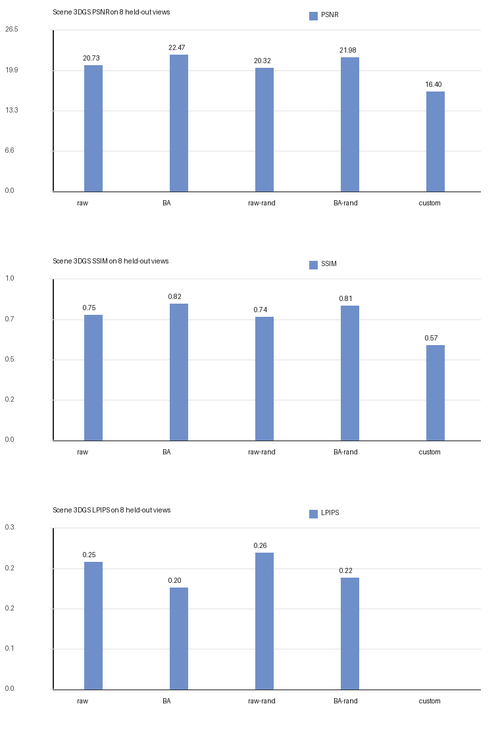
\includegraphics[width=0.78\linewidth]{scene_gs_metrics.png}
    \caption{\texttt{scene} 场景 3DGS 指标柱状图。BA 后官方 3DGS 在 PSNR、SSIM、LPIPS 上均优于 VGGT raw。}
    \label{fig:gs-metrics}
\end{figure}

\begin{figure}[H]
    \centering
    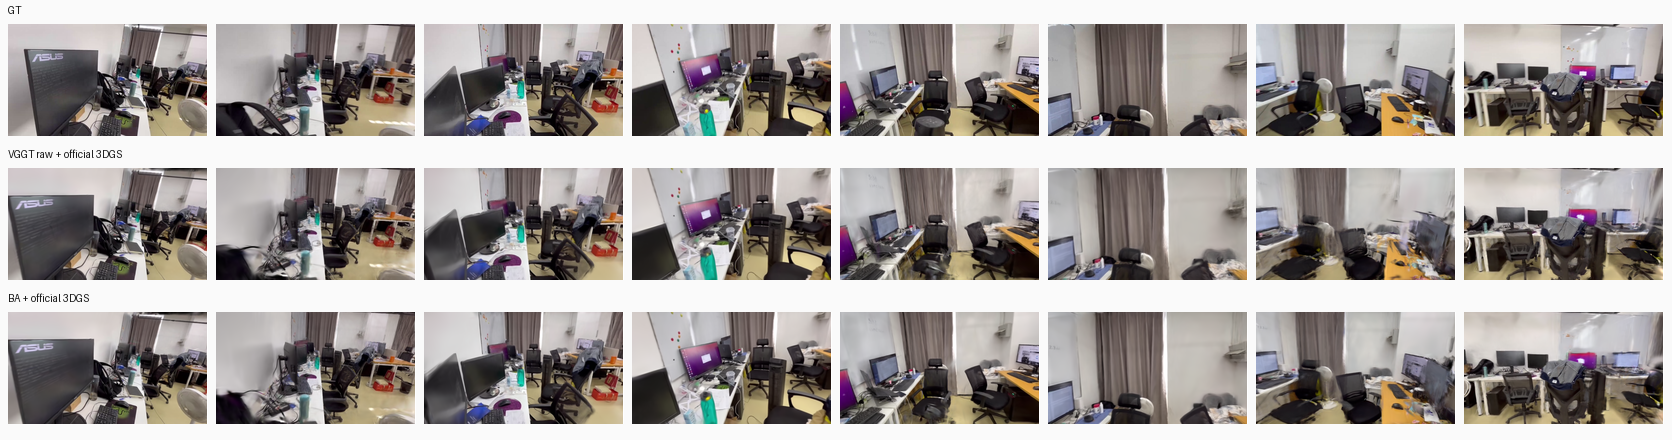
\includegraphics[width=\linewidth]{scene_raw_vs_ba_sheet.png}
    \caption{\texttt{scene} 测试视角渲染对比。第一行为 GT，第二行为 VGGT raw + official 3DGS，第三行为 custom BA + official 3DGS。BA 后椅子、桌面和远处屏幕边缘更稳定，局部漂浮和撕裂减少。}
    \label{fig:scene-raw-ba}
\end{figure}

\begin{figure}[H]
    \centering
    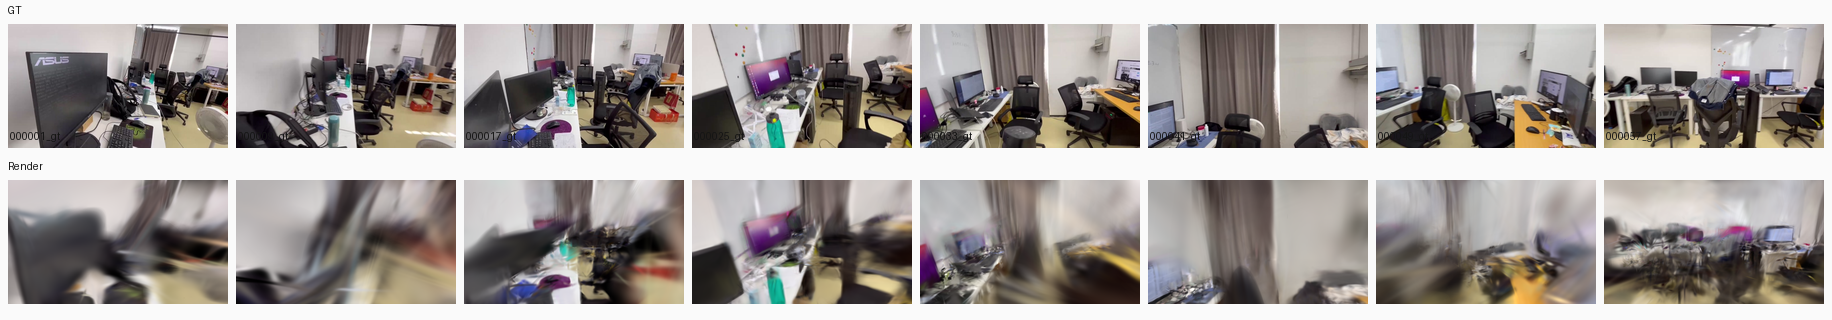
\includegraphics[width=\linewidth]{scene_custom_gt_render_sheet.png}
    \caption{自实现 3DGS 在 \texttt{scene} 上的渲染结果。结果明显模糊，说明当前自定义训练器在 densification、尺度初始化、学习率调度或 renderer 参数上仍有问题。后续主实验采用官方 3DGS。}
    \label{fig:custom-gs}
\end{figure}

\subsection{\texttt{scene\_32} 高密度 tracks 负结果}

由于 human 场景中 query points 数量对结果影响很大，我们进一步尝试在 \texttt{scene} 上验证同样的假设。原始 \texttt{scene} 使用 64 帧图像，为了避免 VGGT/VGGSfM 显存溢出，导出阶段采用 \texttt{max\_query\_pts=512}、\texttt{query\_frame\_num=12}。新的实验使用 FPS=1 采样得到的 \texttt{scene\_32}，将视角数减半以释放显存，并尝试提升 query points 数量。

实验中，\texttt{max\_query\_pts=2048} 和 \texttt{1024} 在 fine tracking 阶段均发生 OOM；最终可稳定运行的配置为 \texttt{max\_query\_pts=768}、\texttt{query\_frame\_num=16}、\texttt{fine\_tracking=true}。该配置确实提高了稀疏点数量：raw track 点从 64 帧 baseline 的 9,760 增加到 16,405，但观测数仍与原配置接近（109,823 vs 116,725），说明减少视角数抵消了单帧 query points 增加带来的观测覆盖收益。

\begin{table}[H]
\centering
\caption{\texttt{scene\_32} 高密度 tracks 实验结果。}
\label{tab:scene32-hq}
\begin{tabular}{lrrrrr}
\toprule
配置 & 图像数 & Raw点数 & BA后RMSE(px) & PSNR$\uparrow$ & LPIPS$\downarrow$ \\
\midrule
\texttt{scene} 原配置 + BA & 64 & 9,760 & 1.58 & 22.47 & 0.197 \\
\texttt{scene\_32} raw, 768 pts & 32 & 16,405 & -- & 18.23 & 0.317 \\
\texttt{scene\_32} BA, 768 pts & 32 & 16,405 & 1.40 & 19.74 & 0.265 \\
\bottomrule
\end{tabular}
\end{table}

该结果说明，在 \texttt{scene} 场景中，简单地用更少视角换取更多 query points 并没有提升 3DGS，反而由于视角覆盖减少导致测试视角泛化更差。BA 在 \texttt{scene\_32} 内部仍然有效，PSNR 从 18.23 dB 提升到 19.74 dB，LPIPS 从 0.317 降到 0.265；但它仍明显低于 64 帧原配置的 22.47 dB / 0.197 LPIPS。因此后续主实验继续使用原始 64 帧 \texttt{scene} 配置，\texttt{scene\_32} 仅作为显存受限下的负结果和消融分析记录。

\subsection{Human 场景问题修复与结果}

初始 human 实验暴露出三个问题：官方仓库默认 LLFF hold-out 规则为每 8 张取 1 张测试图，16 张图像的数据集只有 2 张 test 视角；绿色背景在图像损失和 SSIM 中占比过高；早期 \texttt{1-human} BA 使用的 VGGT 版本与最新 raw 结果不完全一致。针对这些问题，当前代码和实验做了三项修复：

\begin{enumerate}[leftmargin=2em]
    \item 在官方 3DGS wrapper 中写入显式 \texttt{sparse/0/test.txt}，使用 \texttt{TEST\_EVERY=2} 固定 8 张 test 视角。
    \item 使用 \texttt{masks/} 将 human 图像背景合成为白色，并开启官方 3DGS 的 white background。
    \item 在官方 3DGS 初始化前按 mask 过滤点云和观测，同时用更高密度 VGGSfM tracks 重跑 BA。
\end{enumerate}

后续检查表明，human 场景提升的主因并不是 mask 本身，而是 VGGSfM tracks 的 query points 数量。mask 的主要作用是让训练/测试图像背景一致、固定 8 个 test 视角，并过滤明显落在背景区域的点；它可以让指标更稳定，但不能单独补足人体前景的几何覆盖。真正改变重建质量的是高密度 tracks：\texttt{1-human} 从早期约 7.7k 点、57k 观测提升到 18.2k 点、139k 观测，\texttt{2-human} 从约 7.4k 点、59k 观测提升到 17.7k 点、144k 观测。点云和观测数增加后，BA 有更多可靠约束，3DGS 初始化也覆盖了更多人体表面区域，因此渲染质量明显提升。

这个结论对 \texttt{scene} 场景也有启发，但不能直接照搬。Human 数据只有 16 张图，适当增加 query points 可以显著补充前景人体表面；而 \texttt{scene} 的 64 帧原配置已经提供了更完整的视角覆盖。\texttt{scene\_32} 实验表明，在显存限制下只能稳定提高到 \texttt{max\_query\_pts=768}，点数增加不足以弥补视角数减半带来的覆盖损失。因此后续 \texttt{scene} 仍采用原始 64 帧配置作为主实验设置。

\begin{table}[H]
\centering
\caption{Human 场景修复后的官方 3DGS 结果。测试集为显式固定的 8 个 masked-white hold-out 视角。}
\label{tab:human-gs}
\begin{tabular}{lrrrr}
\toprule
场景 & Test视角数 & PSNR$\uparrow$ & SSIM$\uparrow$ & LPIPS$\downarrow$ \\
\midrule
\texttt{1-human} & 8 & 26.44 & 0.959 & 0.031 \\
\texttt{2-human} & 8 & 28.62 & 0.968 & 0.024 \\
\bottomrule
\end{tabular}
\end{table}

\begin{figure}[H]
    \centering
    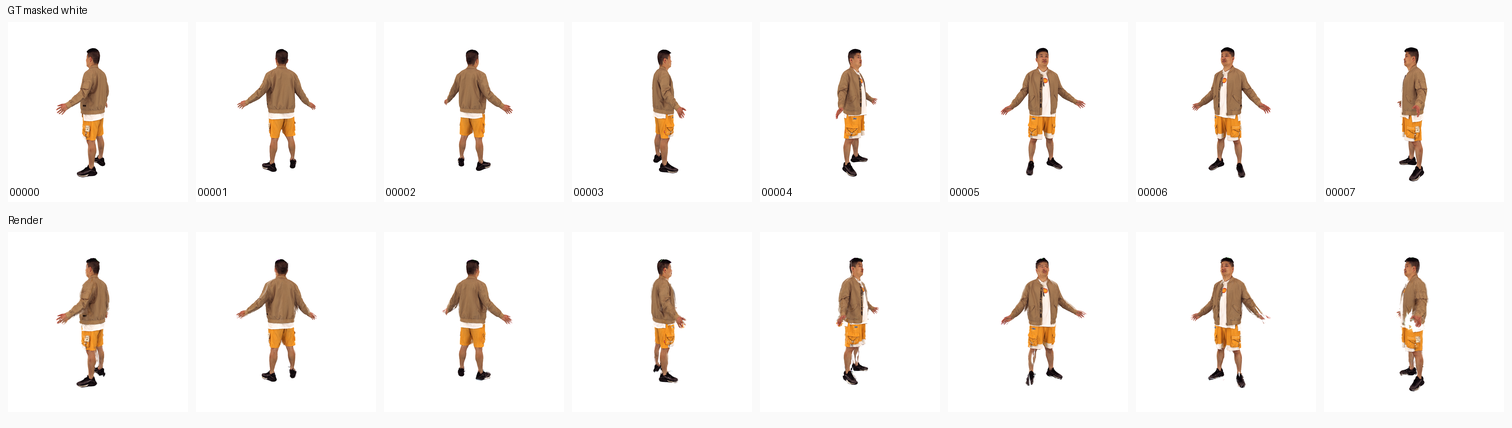
\includegraphics[width=\linewidth]{human1_hq_masked_gt_render_sheet.png}
    \caption{\texttt{1-human} 修复后的 8-view 测试渲染。第一行为 masked-white GT，第二行为官方 3DGS 渲染。}
    \label{fig:human1-render}
\end{figure}

\begin{figure}[H]
    \centering
    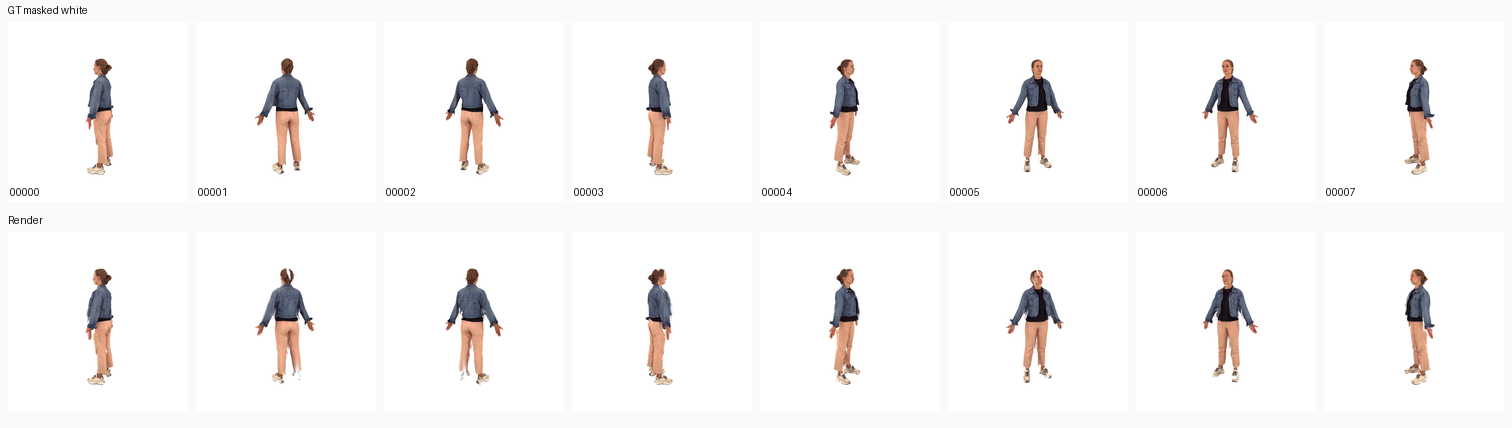
\includegraphics[width=\linewidth]{human2_hq_masked_gt_render_sheet.png}
    \caption{\texttt{2-human} 修复后的 8-view 测试渲染。}
    \label{fig:human2-render}
\end{figure}

修复后的 human 渲染已经可以作为报告展示结果。需要注意的是，这里的指标是在 masked-white 图像上计算，主要评估人体前景重建质量，不再与绿色背景原图指标直接可比。

\section{当前 Pipeline 检查结论}

当前 pipeline 的可交付状态如下：

\begin{itemize}[leftmargin=2em]
    \item \textbf{\texttt{scene}：基本满足报告主实验要求。} VGGT、custom BA、official 3DGS raw/BA 对比、8 张 test 可视化和 PSNR/SSIM/LPIPS 指标均已齐全。额外的 \texttt{scene\_32} 高密度 tracks 实验没有超过原 64 帧配置，因此后续主线继续使用原配置。
    \item \textbf{自实现 BA：可展示。} 三个场景均显著降低重投影误差；高密度 human BA 也已经正常收敛。
    \item \textbf{自实现 3DGS：不适合作为最终效果。} 当前仅在 \texttt{scene} 展示失败结果，后续报告以官方 3DGS 为主要渲染器。
    \item \textbf{human 场景：已得到可展示初版结果。} 通过高密度 tracks、mask 白底合成、mask 点云过滤和 8-view split，两个 human 场景均产出了完整指标和可视化。
\end{itemize}

\section{下一步优化与补实验计划}

在暂不考虑 VGGT 方法改进的前提下，优先补齐以下内容：

\begin{enumerate}[leftmargin=2em]
    \item \textbf{补 raw vs BA 的 human 3DGS 对比。} 当前 human 修复结果主要是 BA 初始化。最终报告可再补 raw high-density 初始化的 masked-white 官方 3DGS，用来直接验证 BA 对 human 3DGS 的影响。
    \item \textbf{补 random init 对比。} 在相同 masked-white split 下跑 random 初始化，区分点云初始化质量和相机/图像预处理的贡献。
    \item \textbf{补前景 mask 指标。} 目前 PSNR/SSIM/LPIPS 在 masked-white 图上计算，后续可进一步只在 mask 前景区域统计，避免白色背景继续抬高指标。
    \item \textbf{清理失败 run 和整理结果索引。} 本轮探索中保留了早期 mask 过滤失败 run 和 \texttt{scene\_32} OOM run；最终归档时应只保留用于报告的明确 run，并在表格中写明 run path。
\end{enumerate}

\section{结论}

本阶段已经完成从 VGGT 到 BA 再到 3DGS 的端到端框架，并在 \texttt{scene} 场景上得到完整、可解释的结果：BA 不仅把重投影 RMSE 从 3.82 px 降低到 1.58 px，也使官方 3DGS 的 PSNR 提升 1.74 dB、SSIM 提升 0.066、LPIPS 降低 0.050。这说明在 VGGT 初始几何基础上加入 BA 对下游 Gaussian Splatting 渲染质量有实际帮助。

当前仍需补充的是更完整的消融：human 场景还应补 raw vs BA、random init、mask 前景区域指标等对比。待这些补实验完成后，报告即可扩展为最终答辩版本。

\end{document}
